\documentclass[tikz, border=10pt]{standalone}
\usepackage{tikz}
\usepackage[T1]{fontenc}

% Match the blue from the reference image
\definecolor{diagblue}{RGB}{31, 119, 180}

\begin{document}
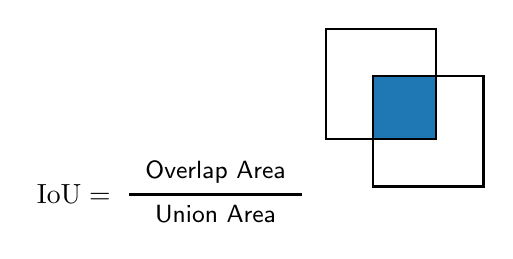
\begin{tikzpicture}[font=\small\sffamily, line width=0.9pt]

% ============================================================
%  PANEL a)  --  formula + visual illustration
% ============================================================

% Fraction bar at y = 1.6
\node[anchor=east] at (1.8, 1.6) {\normalsize$\mathrm{IoU} =$};
\draw[line width=1.2pt] (1.9, 1.6) -- (4.1, 1.6);
\node[anchor=south] at (3.0, 1.6) {Overlap Area};
\node[anchor=north] at (3.0, 1.6) {Union Area};

% ---- Overlap diagram (above bar) ----
% Sq1: (4.4, 2.3) to (5.8, 3.7)   1.4 x 1.4
% Sq2: (5.0, 1.7) to (6.4, 3.1)   offset: +0.6x, -0.6y
% Intersection: (5.0, 2.3) to (5.8, 3.1)
\fill[white] (4.4, 2.3) rectangle (5.8, 3.7);
\fill[white] (5.0, 1.7) rectangle (6.4, 3.1);
\begin{scope}
  \clip (4.4, 2.3) rectangle (5.8, 3.7);
  \fill[diagblue] (5.0, 1.7) rectangle (6.4, 3.1);
\end{scope}
\draw (4.4, 2.3) rectangle (5.8, 3.7);
\draw (5.0, 1.7) rectangle (6.4, 3.1);

\end{tikzpicture}
\end{document}
